\chapter{绪论}



计算机控制技术基础与多门课程相关联,例如:数电、模电、单片机、微机原理、计算机接口技术、自动控制、电机学、运动控制、过程控制等。与其他课程的关系体现在以下几方面:

\begin{itemize}
  \item
输入/输出过程通道:模电、数电、计算机接口技术等;
  \item
计算机/CPU:单片机、微机原理、PLC、DSP、ARM、FPGA等;
  \item
方法及应用:自动控制、运动控制、过程控制、PID、电机学等;
  \item
总线技术:网络技术、USB总线、工业现场总线等。
\end{itemize}




\section{计算机控制系统基本概念}




通俗地讲,利用\textbf{计算机参与控制}的系统称为计算机控制系统。


\begin{table}[h]
  \centering
\begin{tabular}{|c|c|}
  \hline
  % after \\: \hline or \cline{col1-col2} \cline{col3-col4} ...
  模拟控制系统 & 计算机控制系统 \\ \hline
  难以实现复杂规律的调节控制 & 实时数据处理 \\
  不易实现集中监视和操作 & 实时监督决策 \\
  控制方案的更改比较困难 & 实时控制输出 \\
  \hline
\end{tabular}
  \caption{模拟控制与计算机控制系统的对比}\label{tab:1.1}
\end{table}








\section{计算机控制系统的组成}

计算机控制系统由控制计算机和被控对象组成,控制计算机包括硬件和软件两部分:

\begin{itemize}
  \item 硬件:
  \begin{enumerate}
    \item 主机
    中央处理器(CPU)、存储器和接口组成的主机是计算机控制系统的核心。
    \item 过程输入输出设备,
   是主机与被控对象之间的接口,包括模拟量输入输出设备、数字量输入输出设备等。
    \item 人机接口设备
    包括显示器、键盘和打印机等,作用:显示生产过程的状况,供操作员对生产过程发出操作命令,显示操作控制的结果。
    \item 通信设备
  \end{enumerate}


  \item 软件:
  \begin{enumerate}
    \item 系统软件
    可分为通用和专用两类。通用软件指一般计算机使用的软件,如:Windows、VB和Oracle等;专用软件指控制计算机特有的软件,如组态软件。
    \item 应用软件
   是针对某个生产过程编制或生成的专用控制软件。(输入输出、控制算法、人机接口,打印制表)
    \item 管理软件
    实现控制和管理的集成,包括:控制管理、操作管理、经营管理和决策管理等。
  \end{enumerate}

\end{itemize}








\section{计算机控制系统的信号流程}

如图\ref{fig_1_01}所示,计算机控制系统中涉及到以下几种信号:

\begin{figure}[h]
  \centering
  % Requires \usepackage{graphicx}
  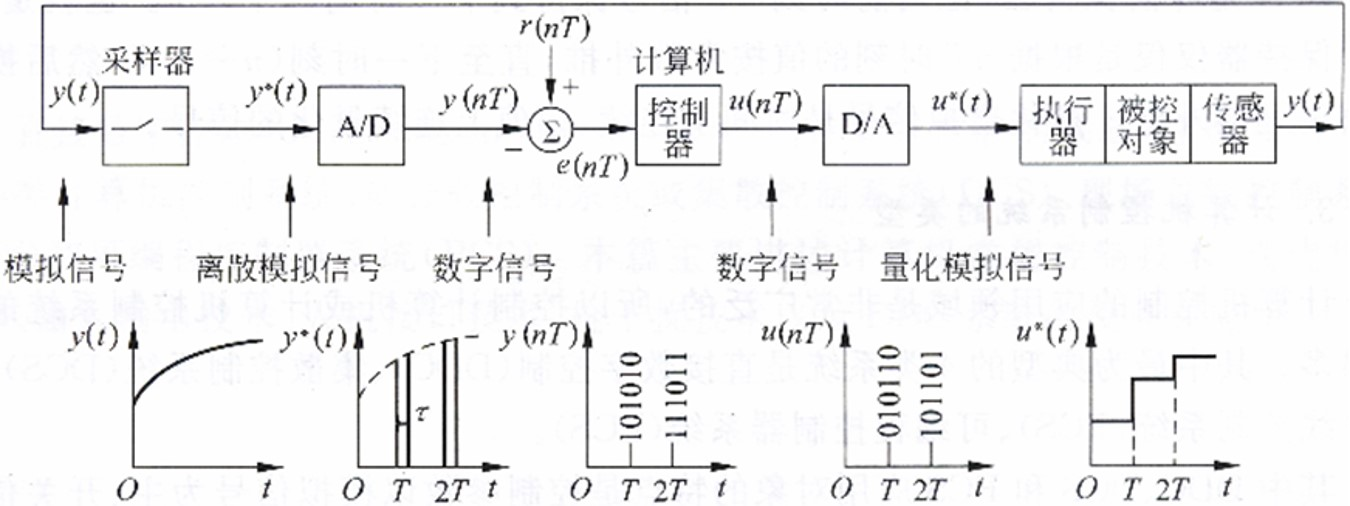
\includegraphics[width=0.8\textwidth]{fig_1_01.jpg}\\
  \caption{计算机控制系统的信号流程}\label{fig_1_01}
\end{figure}


\begin{description}
  \item[模拟信号] 时间与幅值上均连续,如: y(t)、u(t)
  \item[离散模拟信号] 时间离散,幅值连续,如:y*(t)
  \item[数字信号] 时间离散,幅值为数字量,如:y(nT)、u(nT)
  \item[量化模拟信号] 时间连续,幅值为连续量化的信号,如: u*(t)
\end{description}


\section{计算机控制系统分类}

\subsection{按照计算机参与控制的方式}

\begin{itemize}
  \item 开环控制;
  \item 闭环控制。
\end{itemize}

\subsection{按照系统采用的控制规律}


\begin{itemize}
  \item 顺序控制;
  \item 常规控制(PID控制);
  \item 高级控制算法(先进控制、最优控制、自适应控制、预测控制、模糊控制)
  \item 智能控制
\end{itemize}

\subsection{按照计算机应用于工业控制的发展历程及结构特点}



\begin{itemize}
  \item 数据采集系统(DAS:Data Acquisition System)

  \item 操作指导系统(DPS:Data Process System)

  \item 直接数字控制(DDC:Direct Digital Control)

  \item 监督控制系统(SCC:Supervisory Computer Control)

  \item 集散控制系统(DCS:Distributed Control System)

  \item 现场总线控制系统(FCS:Fieldbus Control System )

\end{itemize}

DCS:集散控制系统、分布式、分散型控制;“操作站+工作站+现场仪表”

\begin{itemize}
  \item 计算机价格的下降规律(Intel的摩尔定律:每隔18-24月,计算机性能提升1倍;单位成本下降1/2);
  \item 分散风险;
  \item 构成灵活、积木式、方便替换、维护方便。
\end{itemize}



FCS:现场总线控制系统;随着智能仪表的发展,催生出“工作站+现场总线智能仪表”的系统结构。

\section{本章要点总结}

\begin{enumerate}
  \item 计算机控制系统的概念
  \item 计算机控制系统的组成

  \item 了解计算机控制系统的信号流程
  \item 计算机控制系统的主要类型和各自特点

\end{enumerate}

